Die Darstellung virtueller Szenen durch stereoskopisches Rendering erzeugt die Illusion, dass projizierte Inhalte unter, auf oder über der Bildschirmfläche liegen. Eine konfliktfreie Wahrnehmung der Visualisierung kann durch verschiedene Faktoren eingeschränkt werden. Multi-Touch Eingaben wirken sich durch direkten Kontakt mit dem Projektionssystemen zusätzlichen auf bestehende Probleme aus. In diesem Kapitel werden einige der hervorgerufenen Wahrnehmungskonflikte vorgestellt. Zusätzlich werden bestehende Lösungsansätze aufgezeigt.
\\\\
Abschnitt \ref{sec:related_frame_cancellation} führt hierzu in die Thematik \emph{Frame Cancellation} ein. In Abschnitt \ref{sec:related_touch_interaktion_stereo} werden Probleme und Lösungsbestrebungen beschrieben, welche aufgrund von Touch Interaktion mit stereoskopischen Visualisierungen entstehen. Das Kapitel wird in Abschnitt \ref{sec:diskussion_wahrnehmungskonflikte} durch eine Diskussion dieser verwandten Arbeiten abgeschlossen.


\section{Frame Cancellation}
\label{sec:related_frame_cancellation}

\emph{Frame Cancellation} ist ein Problem, welches in den frühen Jahren der stereoskopischen Filmproduktion von Valyus und Asher erstmals öffentlich benannt wurde \cite{valyus:1966}. Der Wahrnehmungskonflikt entsteht durch eine auftretende Widersprüchlichkeit des Tiefeneindrucks an den Begrenzungen der Projektionsfläche. Bei der Darstellung negativ-parallaxer Inhalte vermittelt die Disparität der Geometrie demnach, dass sich die Darstellung vor dem Bildschirm befindet. Gleichzeitig überlagert dieser durch seine physikalische Begrenzung das Objekt. 
\\\\
Wartell beschreibt eine durch \emph{Frame Cancellation} entstehende schwache Tiefenwahrnehmung der Szene \cite{wartell:2001}. Nach Lipton resultiert außerdem ein unangenehmer visueller Eindruck durch die Schwierigkeit die Bilder der beiden Augen zu vereinigen \cite{lipton:2007}. 
\\\\
Zum Umgang mit diesem Problem, schlägt Autodesk die Verwendung von \emph{Black Bands} vor \cite{autodesk:2008}. Nach diesem Ansatz werden an den äußeren Begrenzungen des Bildes, der jeweiligen Augen schwarze Balken eingeschoben. Abbildung \ref{fig:black_bands} zeigt, dass ohne Anwendung der Technik im Bild des rechten Auges ein kleinerer Ausschnitt der Geometrie zu sehen ist als im rechten. Dieser fehlende Ausschnitt im Bild des linken Auges führt zum beschriebenen Konflikt. Durch Einschieben der \emph{Black Bands} soll die konfliktfreie Verschmelzung der von beiden Augen wahrgenommenen Bilder ermöglicht werden. 

\begin{figure}
	\begin{center}
		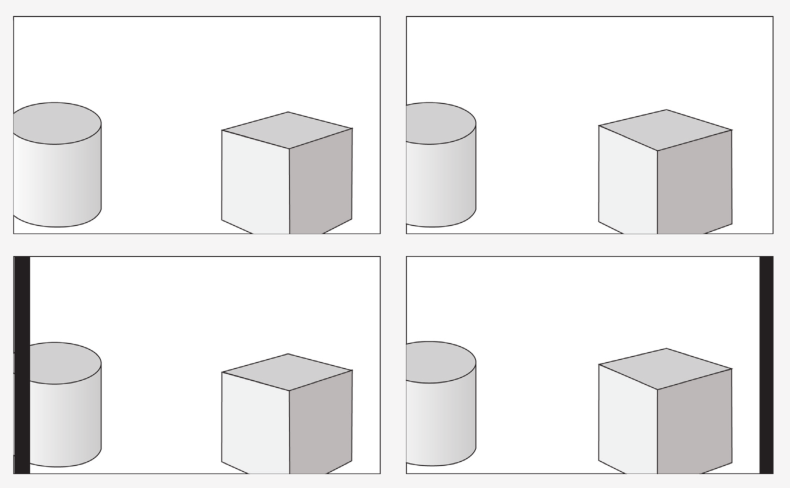
\includegraphics[width=10cm]{img/black_bands.pdf}
	\end{center}
	\caption{Die oberen Abbildungen zeigen die Bildausschnitte der Augen vor Anwendung der \emph{Black-Bands} Technik nach Autodesk \cite{autodesk:2008}. In den darunter liegenden Abschnitten ist die Veränderung dieser nach der Verwendung des Ansatzes zu sehen. Diese Abbildung entstammt vollständig einer Veröffentlichung von Autodesk \cite{autodesk:2008}.}
	\label{fig:black_bands}
\end{figure}

Ardouin et al. schlagen die Verwendung von Clipping zur Begrenzung des Blick Frustums vor \cite{ardouin:2011}. Der Schnittbereich der Frusta beider Augen wird nach Ardouin \emph{Stereo Compatible Volume} genannt \linebreak \cite{ardouin:2011}. In diesem Bereich sei eine konfliktfreie Visualisierung negativ-parallaxer Szeneninhalte sicher. Das Abschneiden der Geometrie außerhalb des Stereo Compatible Volumes (nach Ardouin \emph{Stereo Compatible Volume Clipping}) würde demnach \emph{Frame Cancellation} vermeiden. Abbildung \ref{fig:scvc} zeigt eine Gegenüberstellung der Technik von Ardouin et al. mit \emph{Black-Bands}.

\begin{figure}
	\begin{center}
		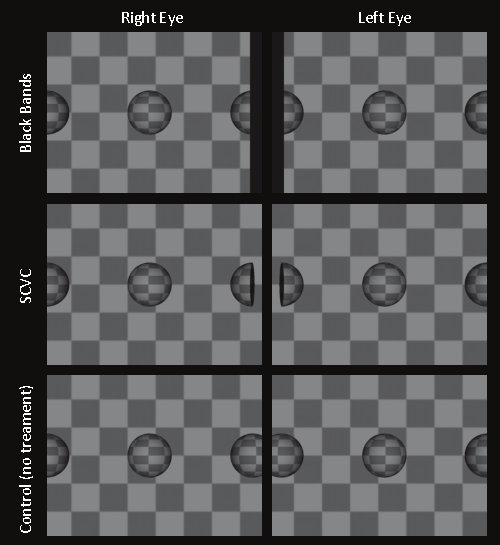
\includegraphics[width=8cm]{img/black_bands_and_SCVC.pdf}
	\end{center}
	\caption{Gegenüberstellung der Techniken \emph{Stereo Compatible Volume Clipping} nach Ardouin et al \cite{ardouin:2011} und \emph{Black-Bands} nach Autodesk \cite{autodesk:2008}. Zum Vergleich wird eine unveränderte Darstellung der Bildausschnitte gezeigt. Diese Abbildung entstammt vollständig einer Veröffentlichung von Ardouin \cite{ardouin:2011}.}
	\label{fig:scvc}
\end{figure}


\section{Touch Interaktion mit stereoskopischen Visualisierungen}
\label{sec:related_touch_interaktion_stereo}

Bei der Touch Interaktion ist die Selektion und Manipulation von virtuellen Objekten auf und abseits der Projektionsebene ausschließlich durch Eingaben auf der Tischebene zu erreichen. Daraus leitet sich eine Wahrnehmungsdiskrepanz ab \cite{valkov:2011,bruder:2013}. Demnach ist die Wahl des Fokuspunktes für die Beobachtung des Interaktionsvorgangs doppeldeutig. Ein Objekt in Negativ-Parallaxe liegt oberhalb der Tischebene, sodass bei Fokussierung von selbigem die Blickrichtung der beiden Augen über der Projektionsfläche konvergiert. Die Wahrnehmung der interagierenden Hand auf dem Bildschirm würde folglich verschwimmen. Umgekehrt würde die Wahrnehmung des parallaxen Inhalts bei Fokussierung der Hand verschwimmen. Abbildung \ref{fig:fokussierung} verdeutlicht diesen Zusammenhang.

\begin{figure}
	\begin{center}
		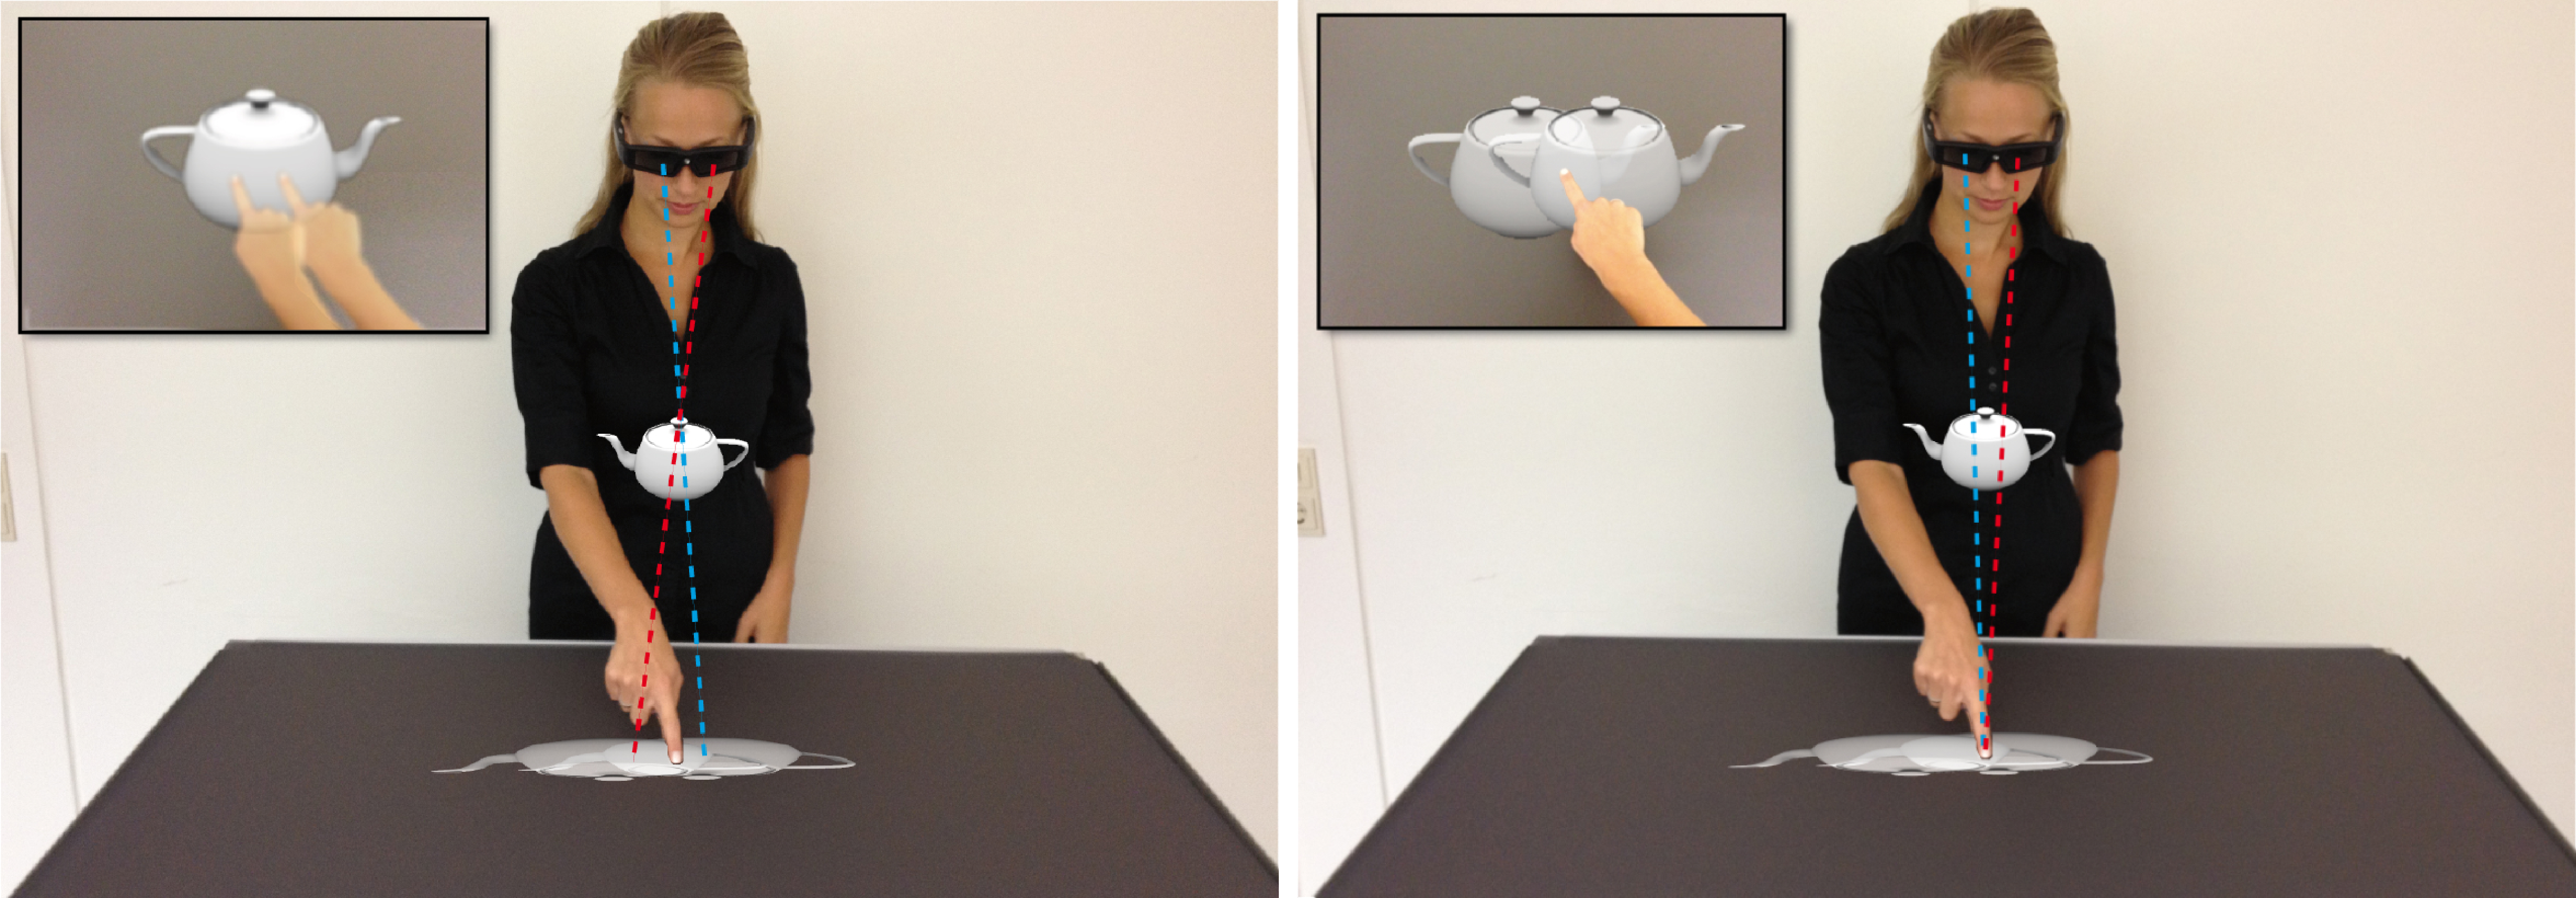
\includegraphics[width=12cm]{img/fokussierung.pdf}
	\end{center}
	\caption{Wahrnehmungsdiskrepanz durch die Wahl des Fokuspunkts. Diese Abbildung entstammt vollständig einer Veröffentlichung von Bruder et al. \cite{bruder:2013}.}
	\label{fig:fokussierung}
\end{figure}

Giesler et al. entwickeln mit ihrer Technik \emph{Void Shadows} einen Ansatz um die Touch Selektion von nicht auf der Bildfläche liegenden Objekten zu erleichtern \cite{giesler:2014}. Hierzu wird eine zweidimensionale Repräsentation aller Geometrie als Schatten auf die Bildebene projiziert. Berührungen eines Schattens werden auf die jeweilig referenzierte Geometrie übertragen.
\\\\
Ein weiteres Problem ergibt sich durch das Eindringen der Hand in über dem Tisch liegende Geometrie. Berührt der Anwender die Tischebene zur Interaktion, durchstößt er dabei die auf dem Pfad der Bewegung liegenden negativ-parallaxen Objekte. Während dem Nutzer durch die Disparität der Darstellung eine geometrische Lage der Inhalte oberhalb der Hand suggeriert wird, bleiben diese verdeckt bis die Hand des Nutzers die Eingabefläche verlässt. Folglich wird die Tiefenwahrnehmung durch die widersprüchliche Lage des projizierten Inhalts in Relation zur Hand des Nutzers gestört. Hierdurch wird der visuelle Eindruck wie bei der \emph{Frame Cancellation} (siehe Abschnitt \ref{sec:related_frame_cancellation}) beeinflusst.
\\\\
Um dieser Problematik entgegenzuwirken verfolgt das von de la Rivière et al. entwickelte System die Bewegung der Hand Nutzer über dem Tisch \linebreak \cite{delariviere:2010}. Nähert sich diese der Tischfläche, wird die Szene entlang der Bildschirmnormalen in Blickrichtung des Nutzers verschoben, bis alle virtuellen Inhalte auf oder unter der Projektionsfläche liegen. Sie verhindern somit mögliche Kollisionen der Hand mit allen dargestellten Objekten.


\section{Diskussion}
\label{sec:diskussion_wahrnehmungskonflikte}

Stereoskopische Projektionssysteme erzeugen durch physikalisch motiviertes Rendering die Illusion einer tatsächlichen Dreidimensionalität der dargebotenen Inhalte. Die in den Abschnitten \ref{sec:related_frame_cancellation} und \ref{sec:related_touch_interaktion_stereo} vorgestellten Konzepte zeigen jedoch, dass die Form der Darstellung, sowie der direkte Umgang mit projizierten Inhalten zu verschiedenen Wahrnehmungskonflikte führen können. Es entsteht dadurch eine Herausforderung für die nutzerfreundliche Zusammenführung mit einem an die zweidimensionale Tischfläche gebundenen Multi-Touch System. 
\\\\
Für die Lösung des \emph{Frame Cancellation} Problems wurde eine Reihe von Ansätzen vorgestellt, welche als sinnvolle Lösungen des Problems zu sehen sind (siehe Abschnitt \ref{sec:related_frame_cancellation}). Die Klärung der von Valkov et al. beschrieben Wahrnehmungsdiskrepanz (siehe Abschnitt \ref{sec:related_touch_interaktion_stereo}) bei Fokussierung von negativ-parallaxen Objekten in Relation zur auf dem Tisch aufgelegten Hand bleibt fraglich.
\\\\
In einer Studie vergleichen Bruder et al. die Präzision der 3D Selektion bei Verwendung von 2D Touch Eingaben mit der freien Auswahl im dreidimensionalen Raum (\emph{3D mid-air} Selektion) \cite{bruder:2013}. Sie kommen zu dem Schluss, dass durch \emph{3D mid-air} Selektion eine höhere Genauigkeit mit schnelleren Interaktionszeiten für Objekte, welche weiter als 10cm abseits der Bildebene liegen, gegeben ist.
\\\\
Die fehlende Effizienz von 2D Touch Eingaben gegenüber \emph{3D mid-air} Techniken könnte durch Ansätze wie \emph{Void Shadows} verbessert werden. Giesler et al. belegen, dass ihre Technik die Präzision und Interaktionszeit, beim Umgang mit vom Bildschirm entfernten Objekten, deutlich verbessert \linebreak \cite{giesler:2014}. Das Anwendungsszenario beschränkt sich bei ihrer Arbeit auf den Umgang mit positiv-parallaxen Inhalten und sollte für Inhalte oberhalb der Tischebene erweitert werden.
\\\\
Die im System von de la Rivière et al. integrierte Funktionalität beseitigt das Auftreten von Wahrnehmungskonflikten durch Eingreifen in virtuelle Modelle \cite{delariviere:2010}. Folgende Kritikpunkte scheinen jedoch naheliegend:

\begin{itemize}
	\item Der eigentliche Wahrnehmungskonflikt wird nicht gelöst. Man vermeidet lediglich die Konfrontation.
	\item Die Translation der Szene ohne direkte Eingabe des Anwenders ist fraglich für die Nutzerfreundlichkeit des Systems.
	\item Das System erlaubt nicht den Umgang mit der Szene in jeder geometrischen Lage
\end{itemize}